\begin{frame}
    \frametitle{AHTR Temperature Model Results}
    \begin{columns}
        \begin{column}{0.6\textwidth}
            \begin{figure}[]
                \centering
                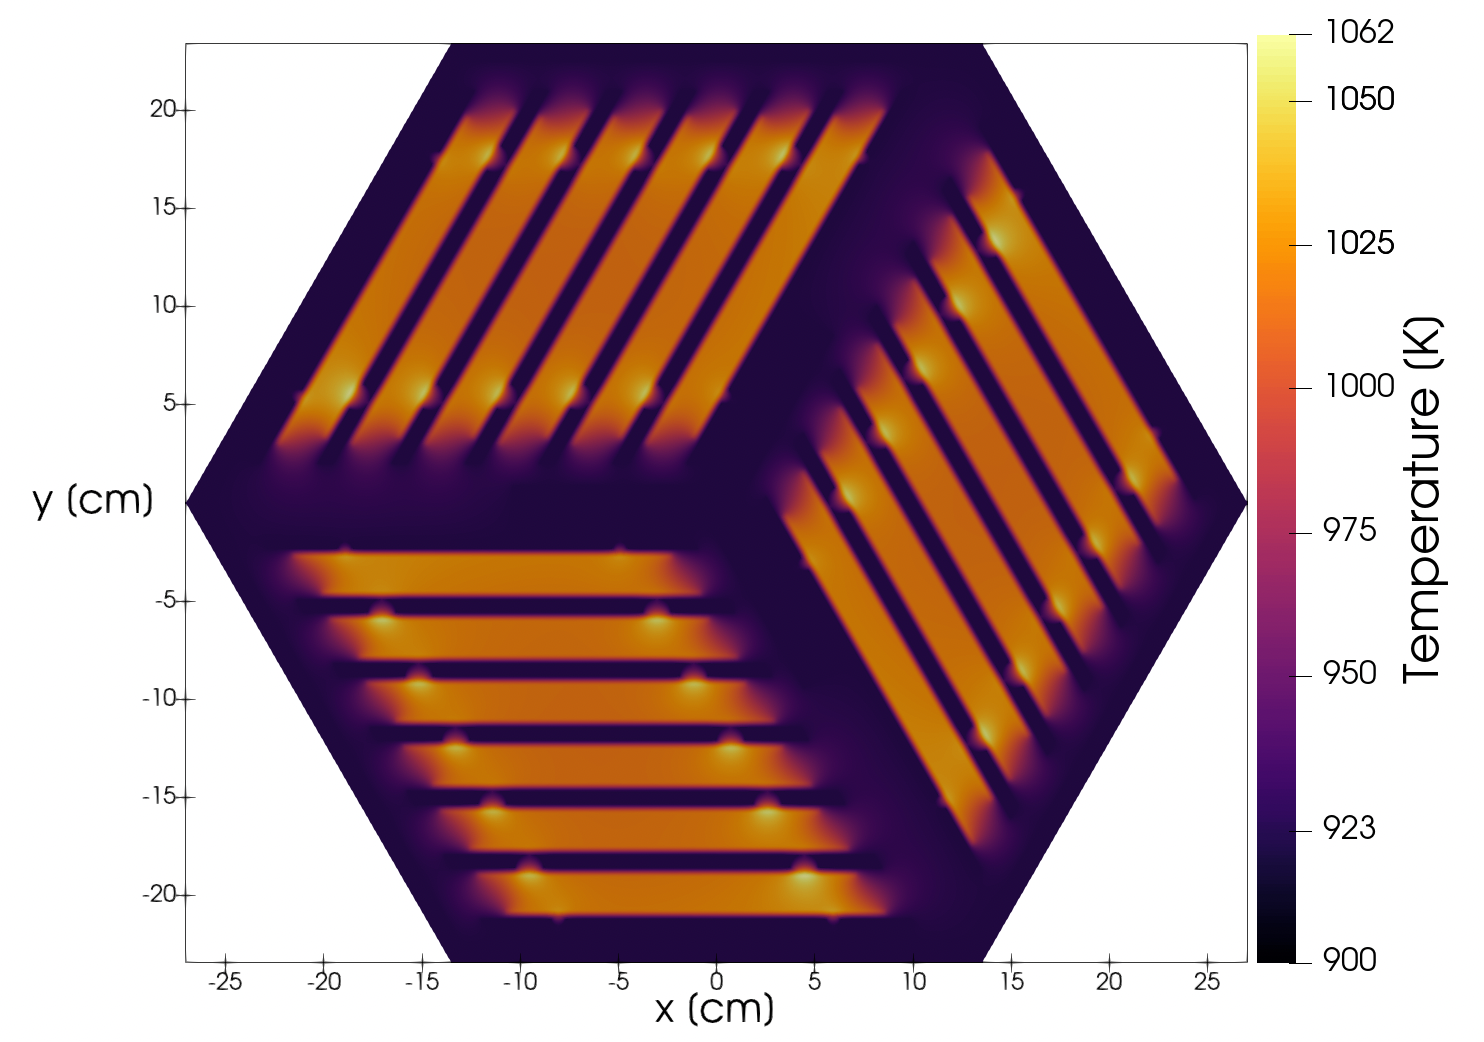
\includegraphics[width=\linewidth]{../docs/figures/benchmark-temperature-model.png} 
                \caption{2D temperature distribution in the \acrfull{AHTR}
                full assembly generated by Moltres.}
            \end{figure}
        \end{column}
        \begin{column}{0.4\textwidth} 
            \begin{block}{Results}
                \begin{itemize}
                    \item Average temperature distribution across the fuel planks are 
                    similar at approximately 1025K
                    \item Graphite structure has an average temperature of approximately 
                    935K
                    \item Temperature peaks at 1062K in the fuel stripes near the spacers
                    \item This could be due to the extra moderation provided by the
                    graphite spacers.
                \end{itemize}
            \end{block}
        \end{column}
        \end{columns}

\end{frame}